\newcommand{\ones}{\mathbf 1}
\newcommand{\reals}{{\mbox{\bf R}}}
\newcommand{\integers}{{\mbox{\bf Z}}}
\newcommand{\symm}{{\mbox{\bf S}}}  % symmetric matrices

\newcommand{\nullspace}{{\mathcal N}}
\newcommand{\range}{{\mathcal R}}
\newcommand{\Rank}{\mathop{\bf Rank}}
\newcommand{\Tr}{\mathop{\bf Tr}}
\newcommand{\diag}{\mathop{\bf diag}}
\newcommand{\card}{\mathop{\bf card}}
\newcommand{\rank}{\mathop{\bf rank}}
\newcommand{\conv}{\mathop{\bf conv}}
\newcommand{\prox}{\mathbf{prox}}

\newcommand{\Expect}{\mathop{\bf E{}}}
\newcommand{\Prob}{\mathop{\bf Prob}}
\newcommand{\Co}{{\mathop {\bf Co}}} % convex hull
\newcommand{\dist}{\mathop{\bf dist{}}}
\newcommand{\argmin}{\mathop{\rm argmin}}
\newcommand{\argmax}{\mathop{\rm argmax}}
\newcommand{\epi}{\mathop{\bf epi}} % epigraph
\newcommand{\Vol}{\mathop{\bf vol}}
\newcommand{\dom}{\mathop{\bf dom}} % domain
\newcommand{\intr}{\mathop{\bf int}}
\newcommand{\sign}{\mathop{\bf sign}}

\newcommand{\cf}{{\it cf.}}
\newcommand{\eg}{{\it e.g.}}
\newcommand{\ie}{{\it i.e.}}
\newcommand{\etc}{{\it etc.}}

\title{Optimal Battery Load Scheduling for Minimizing Energy Costs}
\author{
        Katie Wurman
}
\date{\today}

\documentclass[12pt]{article}
\usepackage{float}
\usepackage{amssymb,amsmath}
\usepackage{graphicx}
\graphicspath{ {figures/} }


\begin{document}
\maketitle

\section{Introduction}
This is a project which simulates a dynamic battery system using real load and solar generation data. The objective is to design a battery load schedule which minimizes total energy costs. Energy costs vary over time and are proportional to the load. The approach in this paper is to simulate the battery as a linear dynamical system with a control input which dictates how much load the battery should absorb or release. The control signal will be computed using an optimal control law, where our objective is cost minimiation and our constraints are the battery dynamics. Results of this approach provide a battery load schedule which stricly reduce energy costs. 

\section{Problem Statement}\label{problem statement}
\paragraph{Billing Schedule}
Energy costs are subject to a time-of-use billing periods and account not just for the quantity of energy consumed but also for the cost to deliver that energy (know as a demand charge). There are three time-of-use periods which affect pricing: peak, part-peak, and off peak. Each period has an energy charge and a demand charge. The enery charge is applied to the total load within the time-of use period. The demand charge is applied to the highest load value within the time-of-use period. A mathematical definition of the energy costs is as follows: 

Define the load data as a vector $v \in \reals^N$ where $N$ is the number of load measurements over the billing period. In this model, measurements are taken every fifteen minutes and the billing period is one week. Define $\alpha_{pk}, \alpha_{pp}, \alpha_{off}$ as the scale factors for the energy cost. Similarly, define $\beta_{pk}, \beta_{pp}, \beta_{all}$ as the scale factors for the demand cost. Then the total energy costs is defined as
\begin{equation}
\begin{split}
J(v) &= \sum_{k=1}^N \big( \alpha_{pk} I_{pk}(k)v_k + \alpha_{pp} I_{pp}(k)v_k+ \alpha_{off} I_{off}(k)v_k \big)  \\
&+ \beta_{pk} \max_{k=1,2..,N} I_{pk}(k)v_k +\beta_{pk} \max_{k=1,2..,N} I_{pp}(k)v_k +\beta_{all} \max_{k=1,2..,N} v_k
\end{split}
\end{equation}
where 
\begin{equation}\label{costfun}
I_{pk}(k)= 
\begin{cases}
    1,& \text{if } k \text{is in the peak period}\\
    0,              & \text{otherwise}
\end{cases}
\end{equation}
The indicator functions$ I_{pp}{k}$ and $I_{off}(k)$ are defined similarly.



\paragraph{Battery Dynamics}
We assume the batter has simple linear dynamics without energy loss. The parameters $\epsilon_{acdc}$ and $\epsilon_{dcac}$ denote the input and output inefficentcies of the battery and we set a maximum output of $P_{max}$ and a maximum capicity of $C_{max}$ on the battery. Denote $s(t)$ as the charge of the battery at time $t$ and denote $u(t)$ as our control input. When $u(t)$ is positive, the battery charges and when $u(t)$ is negative the battery discharges. Then for each time $t \in \{1,...,N\}$ we evolve the system as 
\begin{equation}
\begin{split}
s(t+1) &= s(t) + \epsilon_{acdc} u(t) \\ 
y(t) &=   \epsilon_{dcac} u(t) \\
s(t) & \leq C_{max} \quad t \in \{1,...,N\} \\
u(t) & \leq P_{max} \quad t \in \{1,...,N\}
\end{split}
\end{equation}

\paragraph{Optimal Scheduling}
Next, we will define the control law which will compute the optimal load schedule for the battery in order to minimize costs. We will define this control law as an optimal control problem where we will select a set of inputs $u(0),...,u(N-1)$ which will minimize our objective function $J(\cdot)$. Note that without the battery, our cost is $J(v)$. If we include the battery our cost is $J(v+y)$. Using $u \in \reals^{N-1} $ and $s \in \reals^{N}$ as our variables and $v$ as our load data, we solve the optimization problem
\begin{quote}
    \begin{equation}\label{opteq}
    \begin{array}{ll}
    \mbox{minimize}   & J(v + \epsilon_{dcac} u) \\
    \mbox{subject to} & s(t+1) = s(t) + \epsilon_{acdc} u(t) \quad t \in \{1,...,N\} \\
	& s(N) = 0 \\
    	& s(t) \geq 0 \\ 
	& s(t)  \leq C_{max}  \\
   	& u(t) \geq -P_{max} \\\
	& u(t)  \leq P_{max} \\
  	& v(t) + \epsilon_{dcac} u(t) \geq 0
    \end{array}
    \end{equation}
The last constraint in theis problem $v(t) + \epsilon_{dcac} u(t) \geq 0$ ensures that we are only purchasing from the grid and not selling. 
\end{quote}


\section{Implementation}
To simulate this system and compute the optimal schedule, a Python application called \texttt{battery\_sim} was built utilizing the \texttt{cvxpy} package, which solves convex optimization problems using diciplined convex programming.  

\paragraph{The Data}
The simulation was generated using the provided load and solar data. To compute the net load post solar data, the hourly solar data was evenly distributed across 15-min intervals and subtracted from the raw load data. The routine used to generate the load data can be found in  \texttt{load\_generator.py}.

\paragraph{Utility Rate Generator}
To characterize the time-of-use charges, an indicator matrix $A \in \reals^{NxN}$ was generated such that $[Ax]_k = 0$ if $k$ is not in the rate period and $[Ax]_k  = 1 $ if it is. Four indicator matricies $A_{peak}, A_{part\_peak}, A_{off\_peak}$ and $A_{all\_peak}$ are generated as elements of the \texttt{UtilityRateGenerator} class. The source for this class is located in \texttt{util\_rate\_generator.py}.


\paragraph{Battery Simulator}
Taking as inputs the load \texttt{v} and a utility rate generator \texttt{urg} the battery simulator formulates and solves the optimization problem described in (\ref{opteq}). This simulation and support methods can be found in  \texttt{battery\_simulator.py}.

\section{Results}
To begin, let's run the simulation on some artifical load data, so we can get an intuitive understanding of the model. Assuming a constant load of 150kW we see the following results:

\begin{figure}[h]
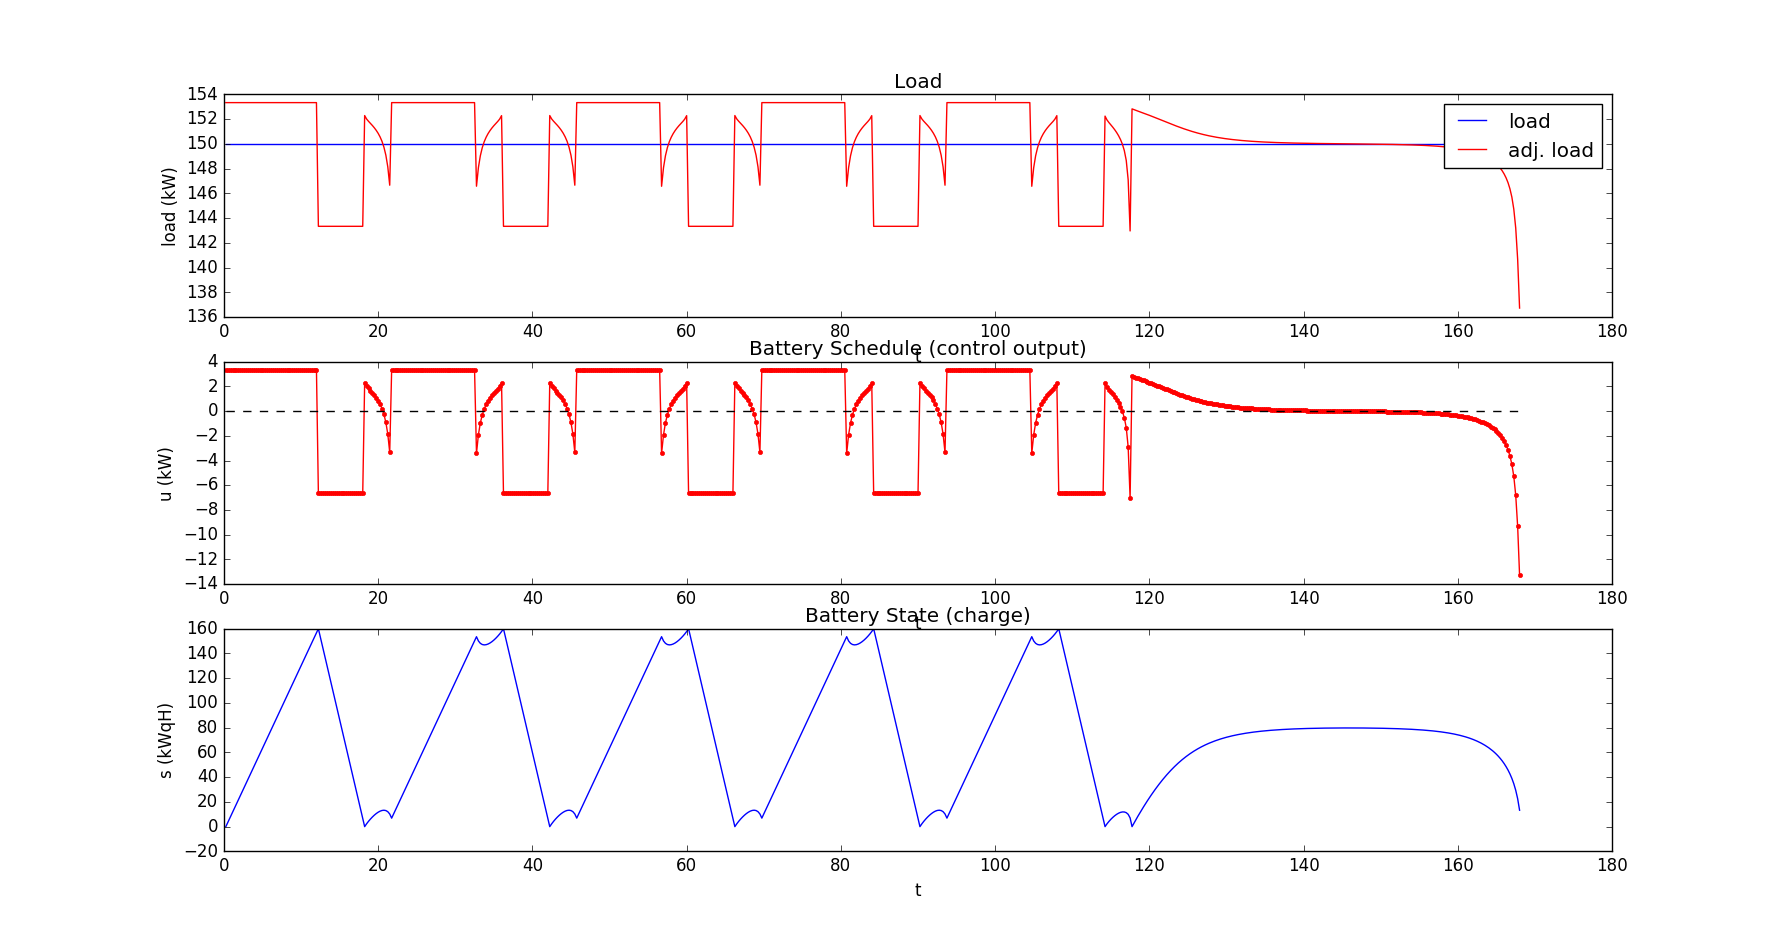
\includegraphics[width=\textwidth]{basicsummary}
\end{figure}
To really see the behaviour, let's look at the battery load super-imposed on the load scaled by the time-of-use cost factors:
\begin{figure}[h]
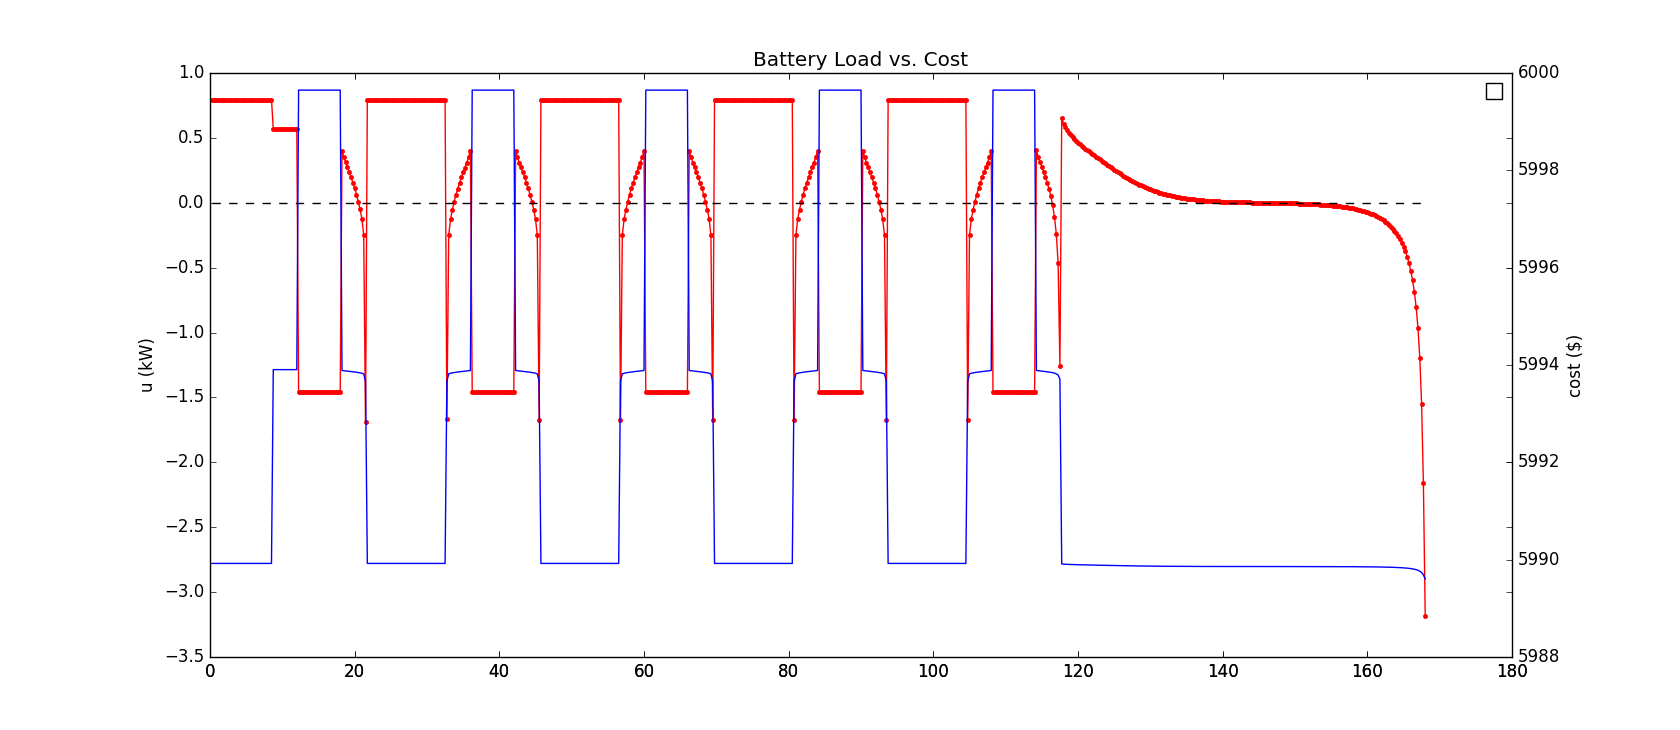
\includegraphics[width=\textwidth]{loadVcost}
\end{figure}
The behavior is aligned: When the cost is lowest, the battery load is highest, which means it's charging. Then when the cost is highest, the battery load is lowest, which means it's discharging. It works! 

Next, let's look at the results of the simulation using the data provided in \texttt{load\_data.csv} and \texttt{generation\_data.csv}:
\begin{figure}[h]
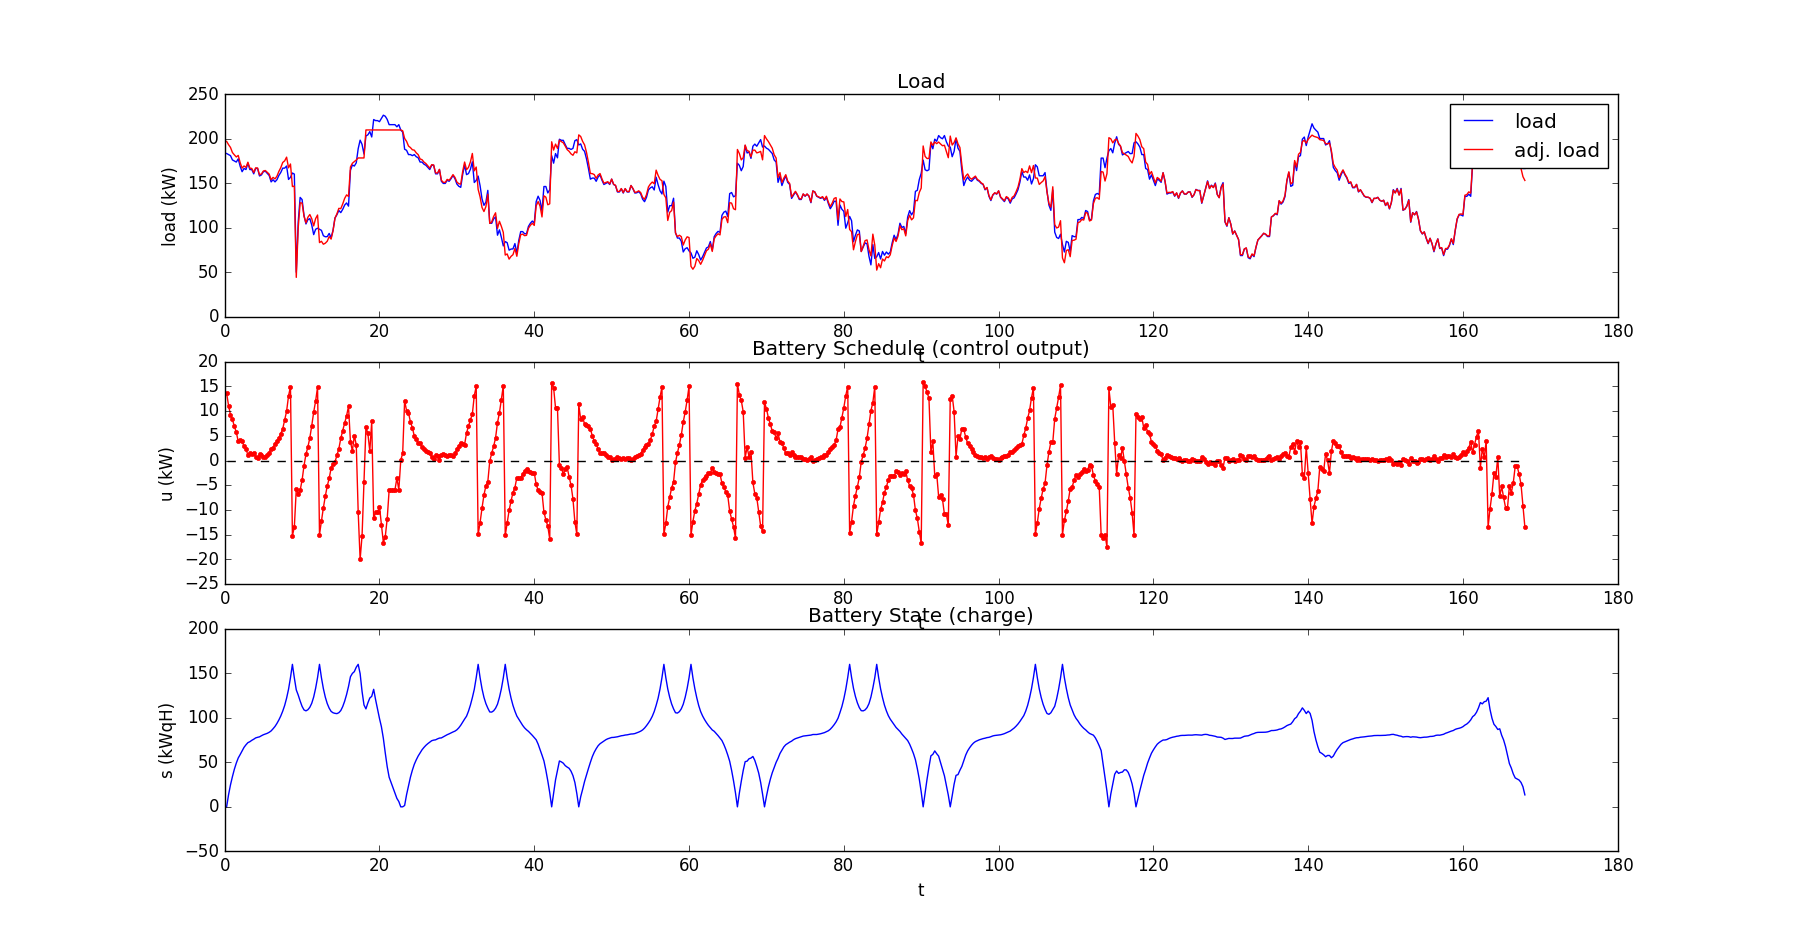
\includegraphics[width=\textwidth]{realsummary}
\end{figure}
 \newline The plots here show a similar charging during low demand periods and discharging during high-demand periods. 


\begin{figure}[H]
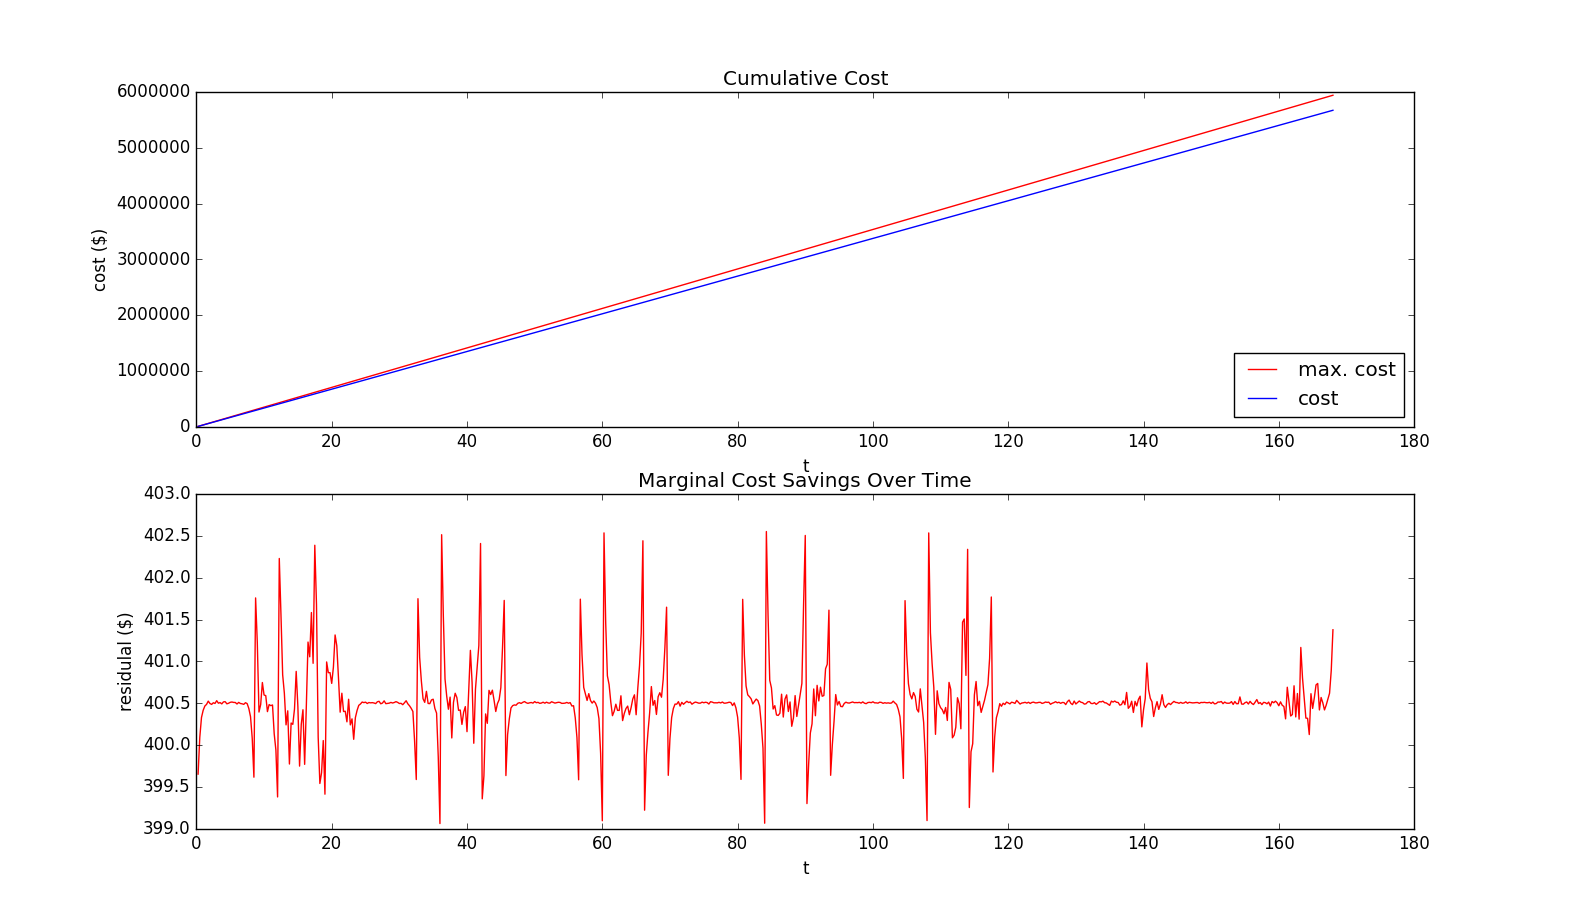
\includegraphics[width=\textwidth]{costsummary}
\end{figure}

\section{Conclusions}\label{conclusions}
We worked hard, and achieved very little.

\bibliographystyle{abbrv}
\bibliography{main}

\end{document}
This is never printed